\subsubsection{Modifikuoto \LIME pritaikymo \gls{ae} aptikimui tikslumo nustatymas}\label{sec:exp:2}

Šio eksperimento tikslas yra nustatyti modifikuoto \LIME pritaikymo \gls{ae} aptikimui (\ref{sec:method:mods}) tikslumą. \LIME branduolio plotis paliekamas pagal numatytus nustatymus ($\omega = 0,75 \cdot \sqrt{n}$, čia $n$ -- požymių skaičius, taigi, $\omega = 0,75 \cdot \sqrt{200} \approx 10,61$) \cite{ribeiroWhyShouldTrust2016}.

Kadangi šis metodas geba aptikti \gls{ae} -- obfuskuotas programas --
\ref{fig:exp2:confusion} pav. pateikiamos dvi klasifikacijos lentelės. Pirmoje (\ref{fig:exp2:confusion:a}) -- klasifikacijos rezultatai, kai obfuskuota programa laikoma kenkėjiška. Antroje (\ref{fig:exp2:confusion:b}) -- išskiriama \textit{obfuskuota} klasė. Kadangi išskyrus šią klasę duomenų rinkinys tampa subalansuotas, klasifikavimo lentelėje pateikiami sveiki skaičiai, atitinkantys modelio prognozuojamų duomenų tai klasei kiekį.

Eksperimento rezultatai (klasifikavimo metrikos) pateikiami \ref{tbl:exp2:metrics2}-oje ir \ref{tbl:exp2:metrics3}-oje lentelėse.
\begin{figure}[h]
    \begin{subfigure}{0.5\textwidth}
        \centering
        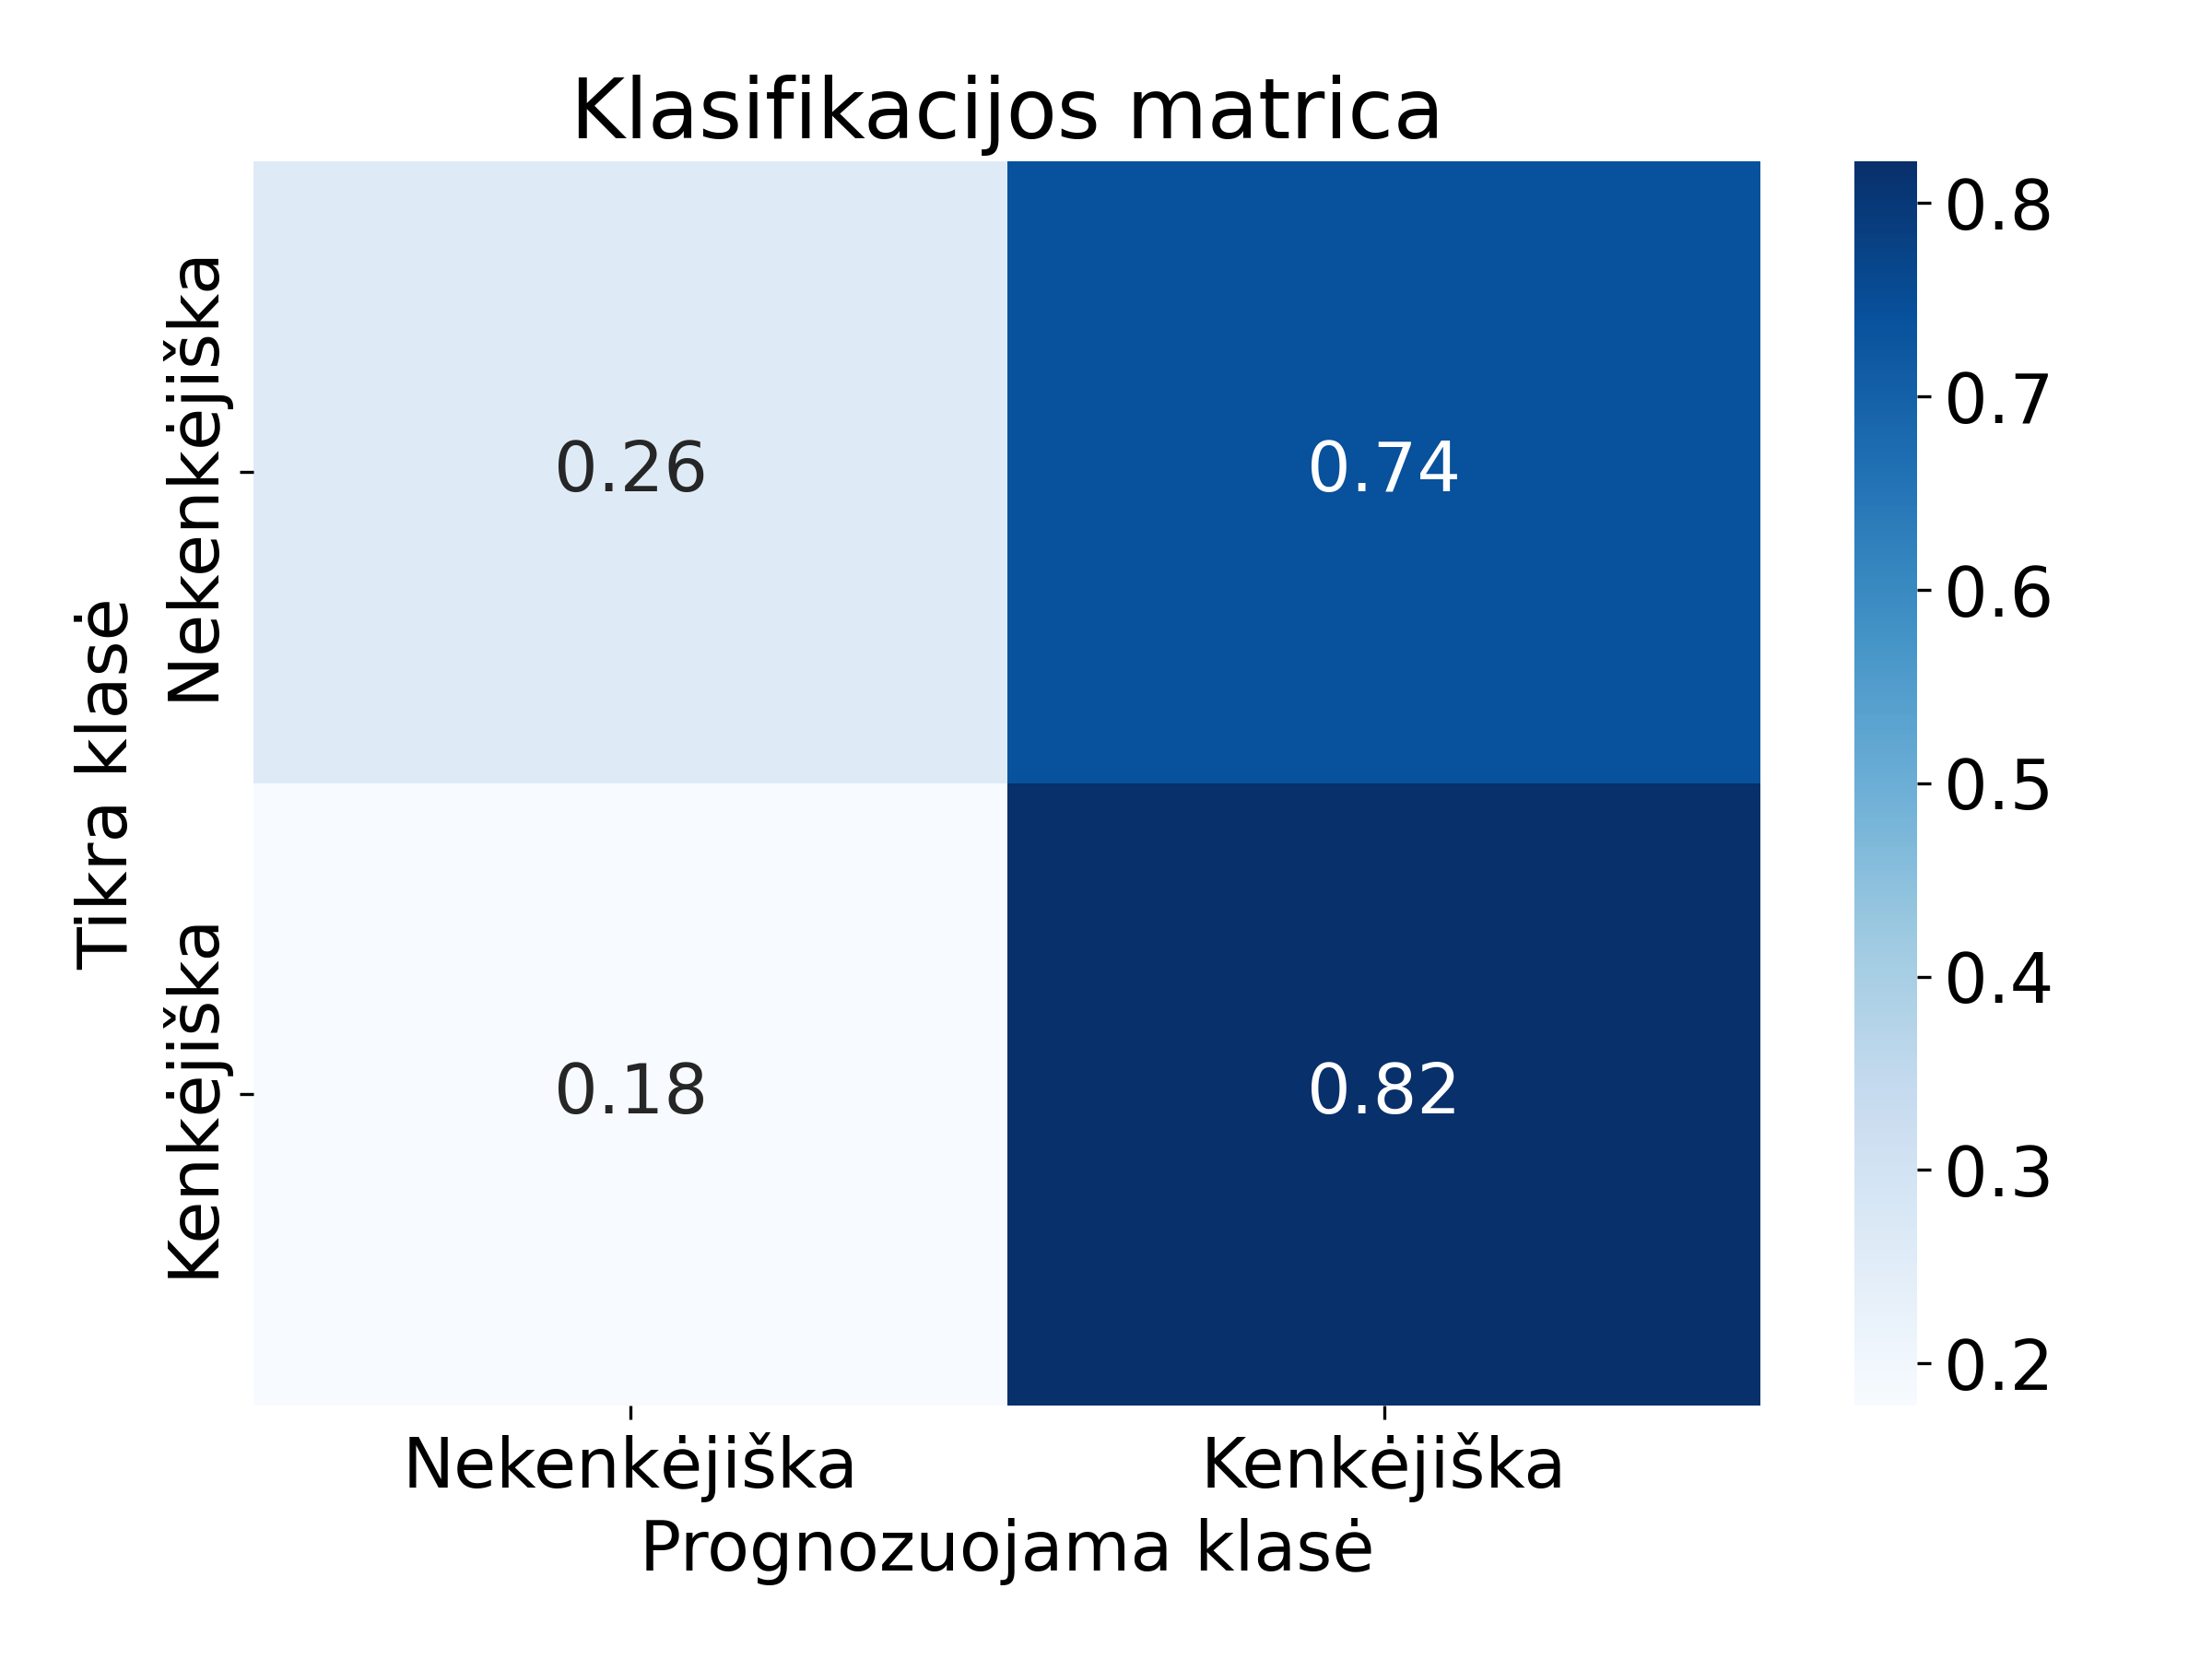
\includegraphics[width=\textwidth]{images/lime_2x2.png}
        \caption{Neišskiriant \textit{obfuskuotų} pavyzdžių klasės}
        \label{fig:exp2:confusion:a}
    \end{subfigure}
    \begin{subfigure}{0.5\textwidth}
        \centering
        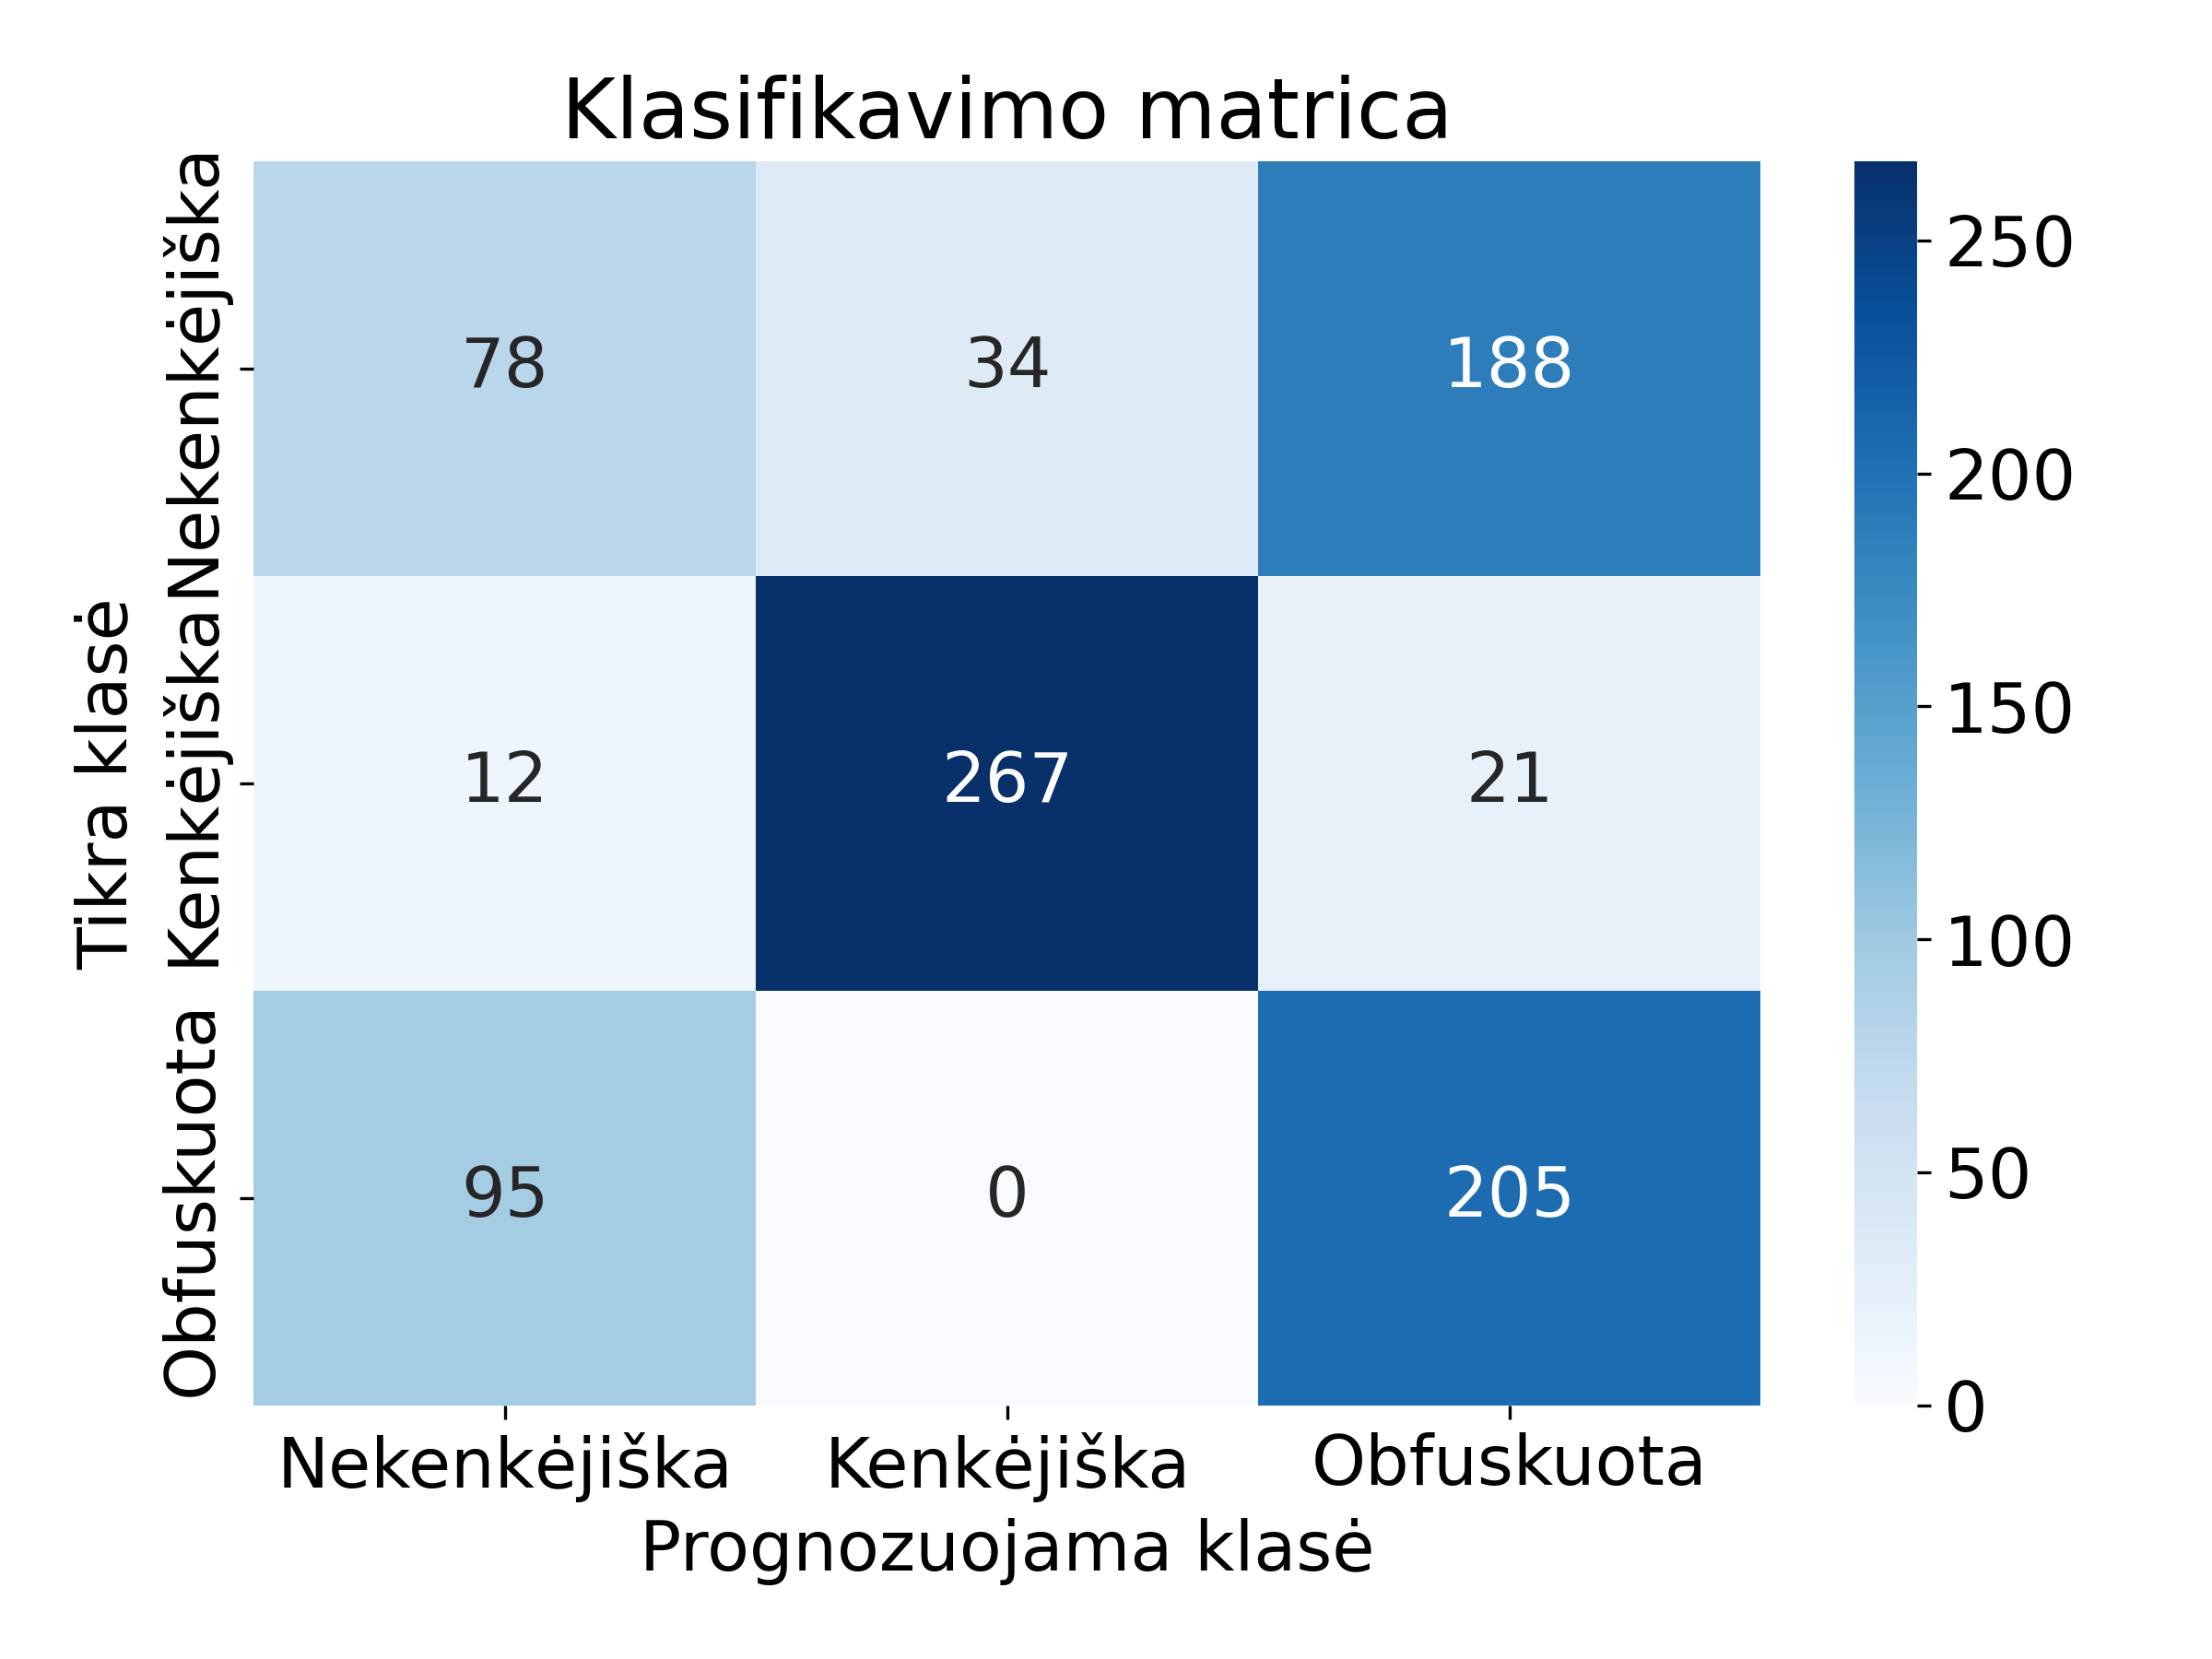
\includegraphics[width=\textwidth]{images/lime_3x3.png}
        \caption{Išskiriant \textit{obfuskuotų} pavyzdžių klasę}
        \label{fig:exp2:confusion:b}
    \end{subfigure}
    \caption{\LIME pritaikymo \gls{ae} aptikimui klasifikavimo lentelės}
    \label{fig:exp2:confusion}
\end{figure}

\begin{table}[h]
    \caption{\LIME pritaikymo \gls{ae} aptikimui klasifikatoriaus metrikos (neišskiriant \textit{obfuskuotos} klasės)}
    \centering
    \exptable[\accLimeCat]{tables/lime_2x2.csv}
    \label{tbl:exp2:metrics2}
\end{table}

\begin{table}[h]
    \caption{\LIME pritaikymo \gls{ae} aptikimui klasifikatoriaus metrikos (išskiriant \textit{obfuskuotą} klasę)}
    \centering
    \exptable[\accLimeCatObf]{tables/lime_3x3.csv}
    \label{tbl:exp2:metrics3}
\end{table}

% Use the paper method and show results that do not perform well